\index{Definition of merge sort}
\justify
{
Merge sort is an efficient sorting algorithm that follows Divide and Conquer algorithm to sort the given list of elements. Technique is recursively divide the given list in two halves until we obtain a certain stage where the length of the list becomes only 1. After that, merge those individual arrays in sorted manner till we combines the total list. Here is a pictorial demonstration available that gives a better understanding with an example of list: [38, 27, 43, 3, 9, 82, 10]\\
}
\index{A merge sort illustration figure}
\begin{figure}[h!]
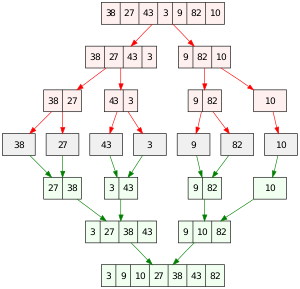
\includegraphics[scale=0.7]{Pictures/300px-Merge_sort_algorithm_diagram.svg.png}
\centering
\caption{Merge sort illustration}
\end{figure}
\index{Steps to sort a list using merge sort algorithm}
Here we take the total list of integers and recursively divide it in two halves until the divided list size becomes 1 then contineously merge them in sorted manner till we reach the exact length as before.
\begin{enumerate}
	\item[Step 1:] [38, 27, 43, 3, 9, 82, 10]
	\item[Step 2:] [38, 27, 43, 3] [9, 82, 10]
	\item[Step 3:] [38, 27] [43, 3] [9, 82] [10]
	\item[Step 4:] [38] [27] [43] [3] [9] [82] [10]
	\item[Step 5:] [27, 38] [3, 43] [9, 82] [10]
	\item[Step 6:] [3, 27, 38, 43] [9, 10, 82]
	\item[Step 7:] [3, 9, 10, 27, 38, 43, 82]
\end{enumerate}
\textcolor{blue}{Yep! the list is sorted.}